%! TEX root = **/010-main.tex
% vim: spell spelllang=en:

\section{Results}

\subsection{Replicating results from Kutznetsov et al.}

To analyze the performance of the program and verify it correctness the parameters found by Kutznetsov et al. \cite{kuznetsov_visualization_2013} are used. \footnote{This system is the same that was previously discussed in~\cref{sec:context} (\cref{fig:kuznetsov})}

Specifically, the following system of equations is studied,
%\Cref{eq:kuznetsov} reports the coefficients used
\begin{equation}%
    \label{eq:kuznetsov}
    \begin{split}
        \frac{dx}{dt} &= x^2 + xy + y^2 + x + y\\
        \frac{dy}{dt} &= ax^2 + bxy * cy^2 + \alpha x + \beta y
    \end{split}
    \qquad \qquad
    \begin{split}
        a &= -10\\
        b &= 2.2\\
        c &= 0.7\\
        \alpha &= -72.7778\\
        \beta &= 0.0015
    \end{split}
\end{equation}

This specific choice of the coefficients is known to result in four limit
cycles, as shown in \cref{fig:kuznetsov2}.

\begin{figure}[H]
    \centering
    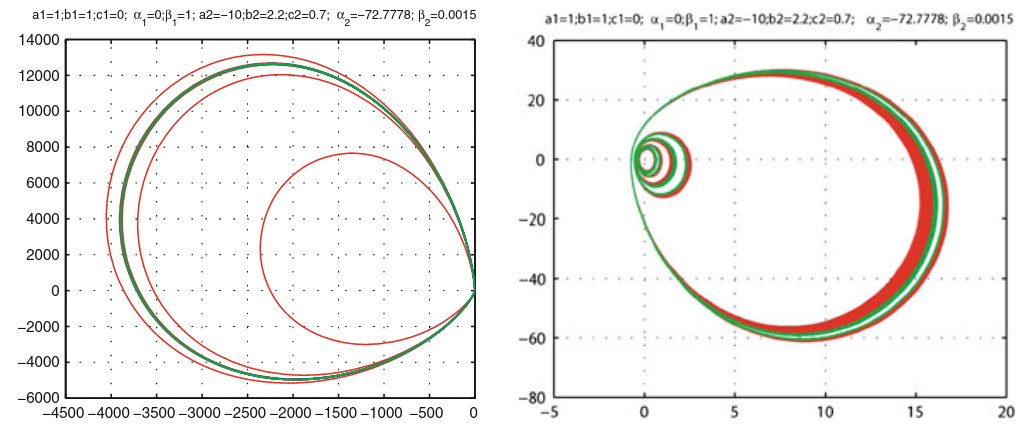
\includegraphics[width=1.0\textwidth]{4cycles}
    \caption{Visualization of four limit cycles in two-dimensional polynomial quadratic system, from Ref.~\cite{kuznetsov_visualization_2013}
    }
    \label{fig:kuznetsov2}
\end{figure}

\pagebreak
\Cref{fig:kuznetsov_cuda} shows a visualization of the points we obtain which a ratio equal to one
{\bf which ratio?}
with tolerance $10^{-6}$.
The coefficients are chosen to be equal to these of Ref.~\cite{kuznetsov_visualization_2013} and their results are reproduced. The computation of this data took 250ms on a grid of $1024 \times 1024$ (i.e. approximately one million of trajectories) using \emph{Runge Kutta} of third order with a step size of $10^{-3}$.
Notice that some of the points from the left part ($x < 0$) of biggest cycle are not found.
% {\bf ??? not clear, rephrase}
Nevertheless, three limit cycles are clearly identified. Notice that the
4th limit cycle which is expected to be present in the left of our plot cannot be found by the program due to the stiffness of the system on that area. This problem is discussed in more detail in~\cref{sub:stiffness}. For the rest of the analysis we will only consider these 3 limit cycles.
\begin{figure}[H]
    \centering
    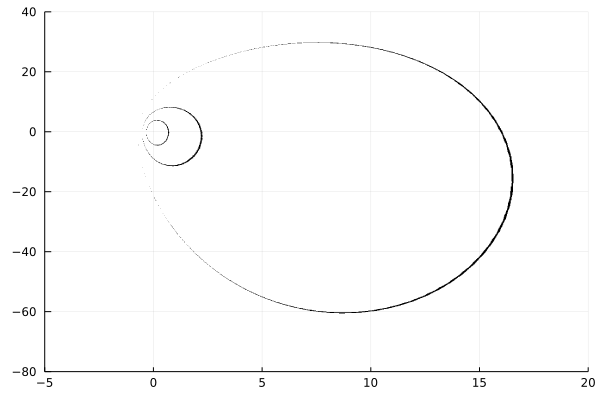
\includegraphics[width=0.8\textwidth]{kutznetsov_cuda}
    \caption{Limit cycles found in the reference case, Eq.~\ref{eq:kuznetsov}, discretizing the phase space by $1024\times 1024$ grid.
    }
    \label{fig:kuznetsov_cuda}
\end{figure}

Using a bigger grid size ($5000\times5000$ initial points), we obtain clearer results and the execution time grows to 1200ms=1.2s.
%There is not much benefit in this instance since the cycles are clear and we are searching inside a well delimited plane, but when the search space is greater it does offer a benefit.
The increase of the resolution does not lead to drastic change in the picture as
the limit cycles were clearly separated on a grid with a smaller resolution.
In~\cref{fig:detail1kvs5k} we can appreciate how having 5 times more resolution on each dimension
gives more detail which could be crucial
%Nevertheless, it might be expected that having high resolution can be crucial
in some other cases in which the limit cycles are not so clearly visible with the specified window.
In~\cref{sub:window_range} there are some examples of some possible situations where resolution is crucial to obtain good results.
%{\bf ??? check last two sentences, did I get it correct?}

\begin{figure}[H]
\centering
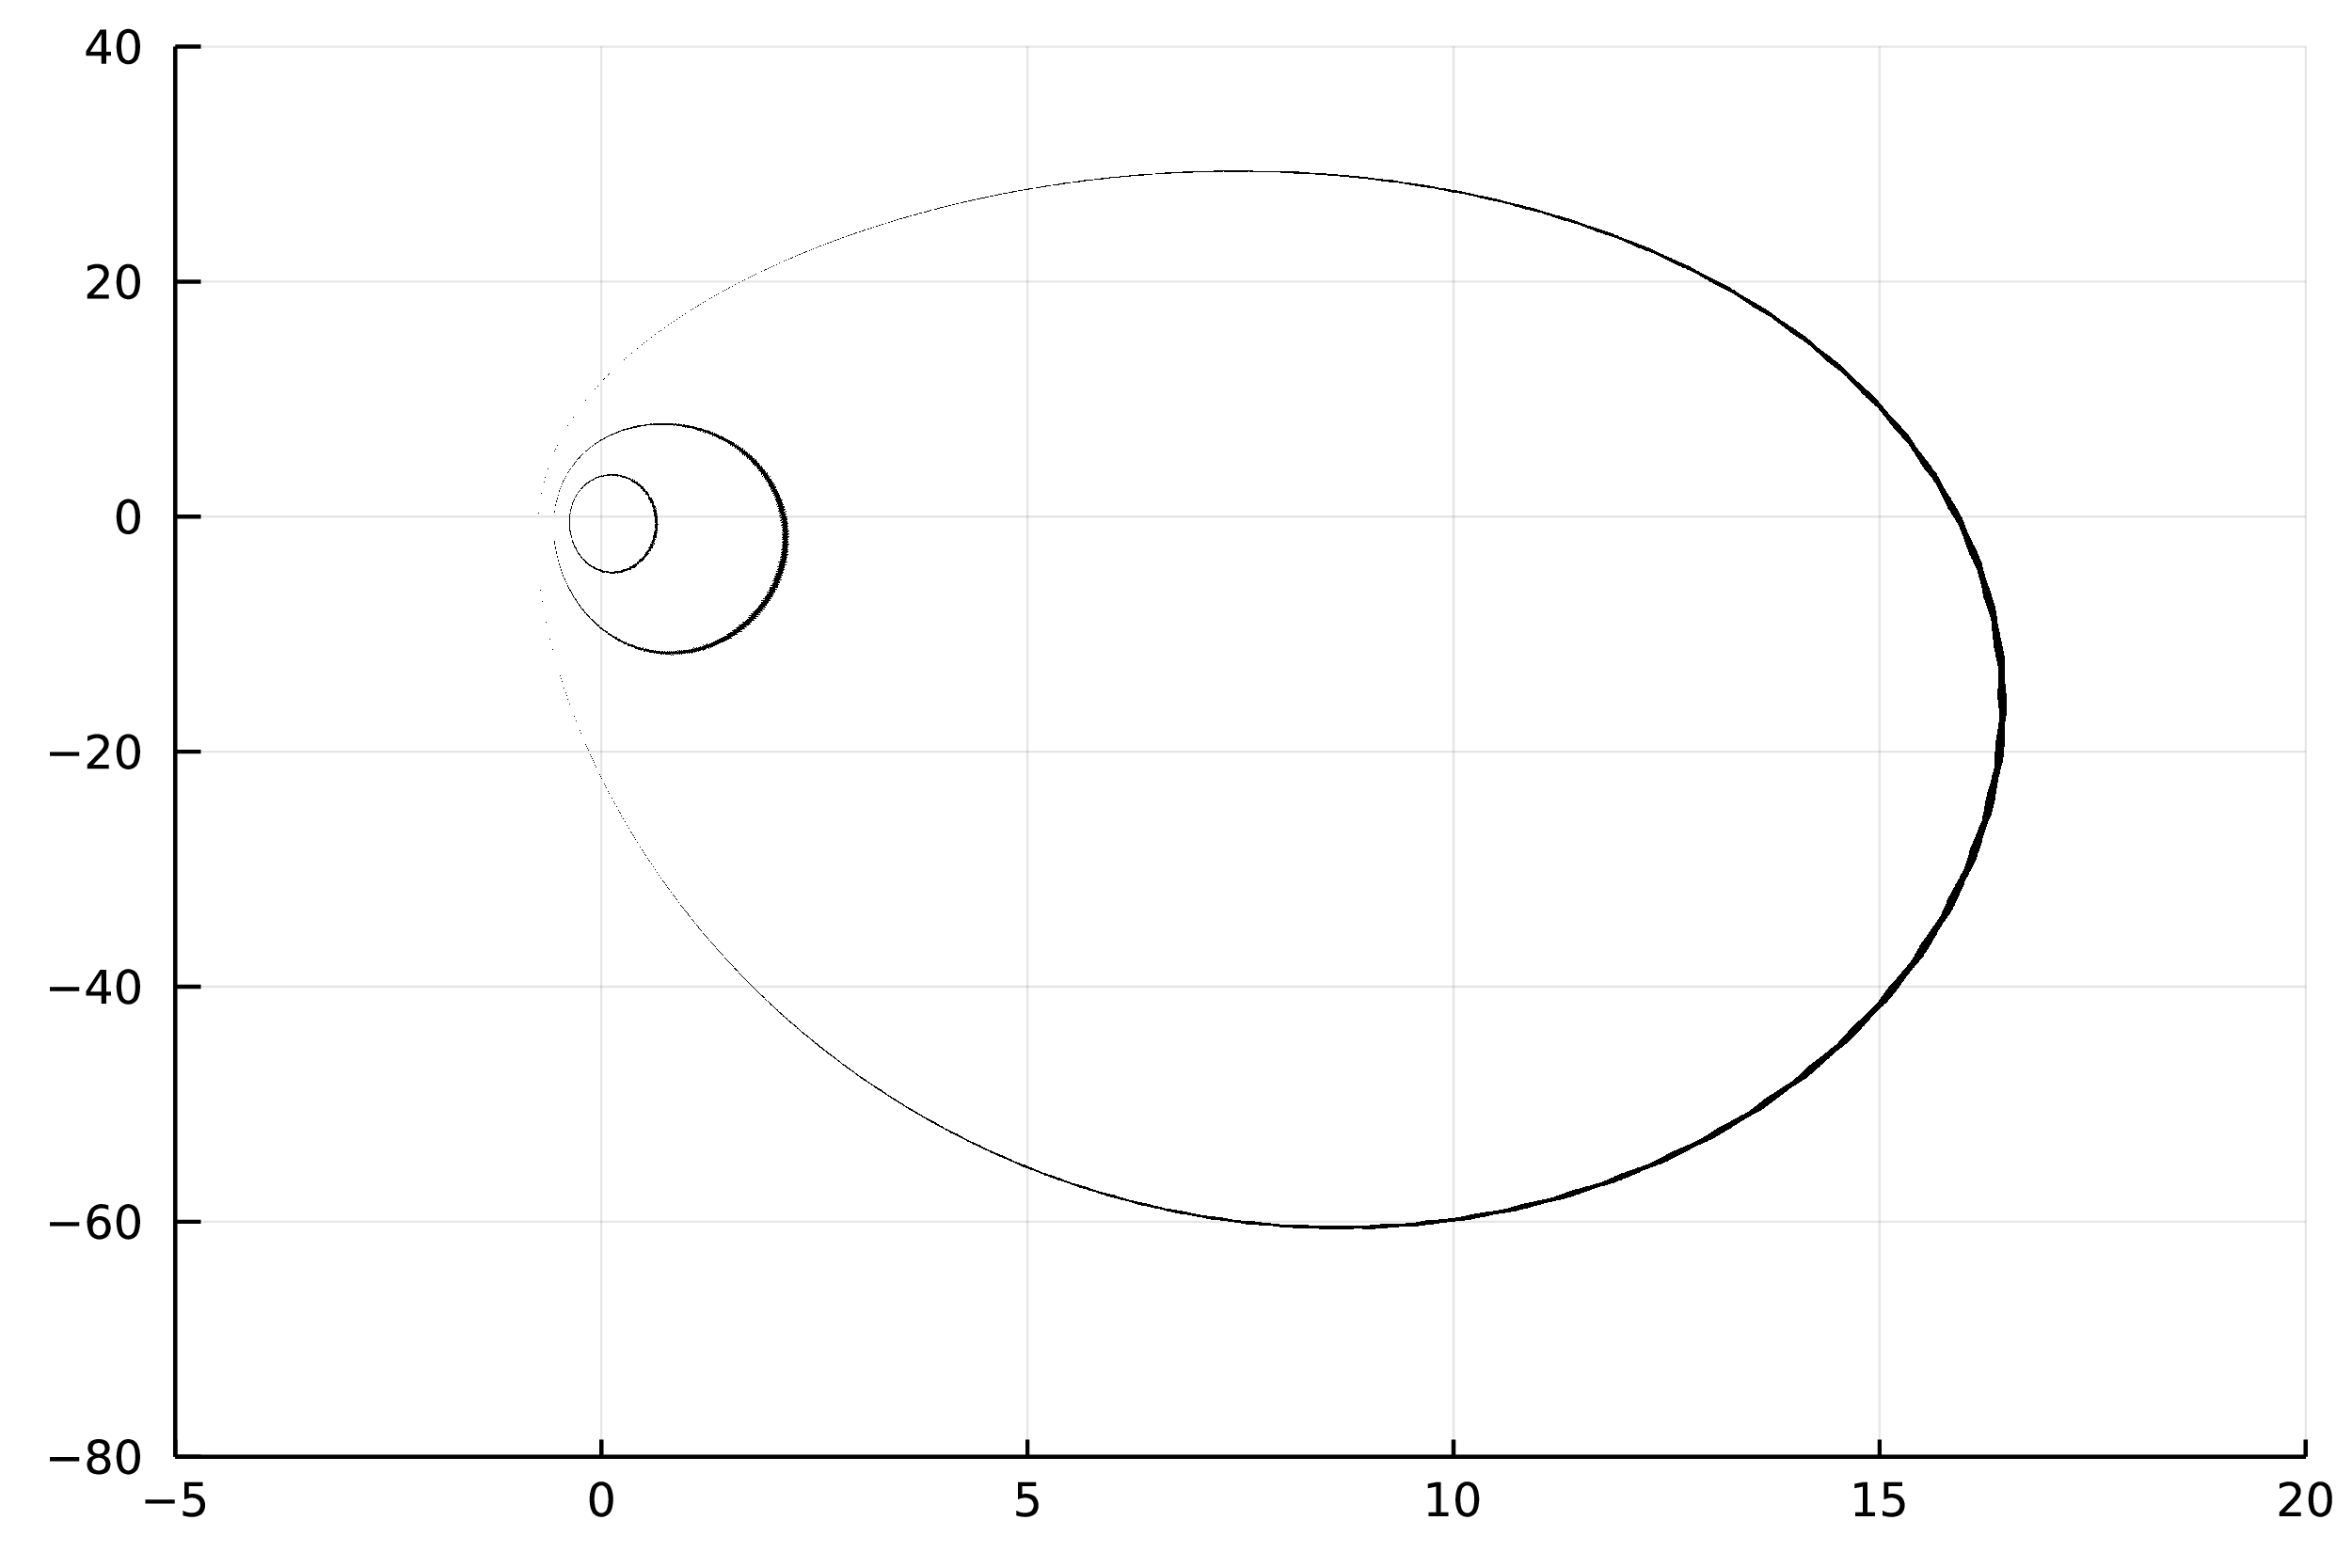
\includegraphics[width=0.8\textwidth]{kutznetsov_cuda_5k}
\caption{Limit cycles found using the developed program ($5000\times 5000$ grid)\\
Black areas correspond to points from which trajectories have a rate of 1 {\bf ??? what is that}  (tolerance $10^{-6}$)
}
\label{fig:kuznetsov_cuda_5k}
\end{figure}

\begin{figure}[H]
\centering
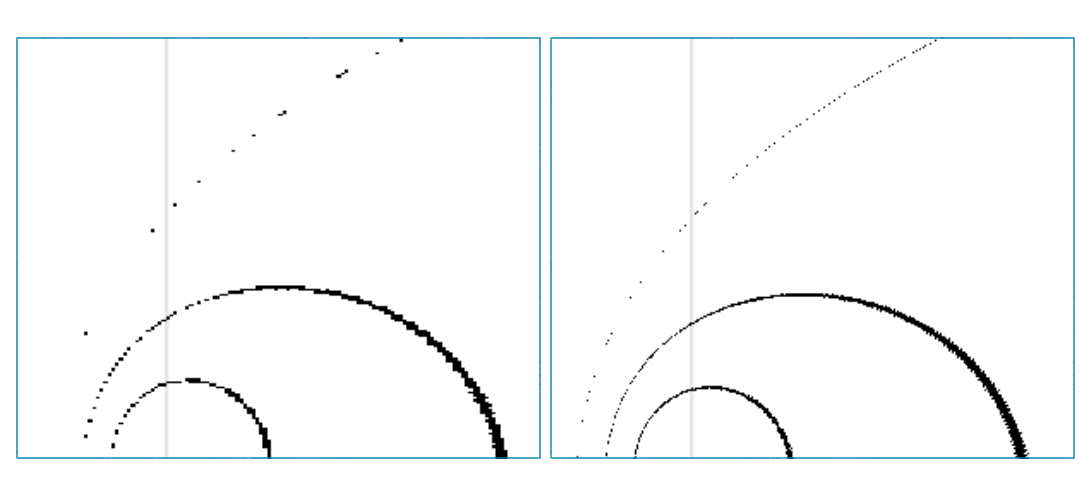
\includegraphics[width=0.8\textwidth]{detail_1000_vs_5000}
\caption{Detail of the same region from \cref{fig:kuznetsov_cuda} (left) and \cref{fig:kuznetsov_cuda_5k} (right)
}
\label{fig:detail1kvs5k}
\end{figure}

\paragraph{Clustering}

\Cref{fig:histograms} shows the histogram of the positions of the four local extrema, that is the maximal and minimal positions of the $x$ and $y$ coordinates.
%4 different local extrema values associated with all points with rate of change equal to 1 (with tolerance $10^{-6}$),
One can clearly see that there 3 groups in each one of the local extrema associated with 3 different limit cycles.
Thus this type of the histogram allows to count the number of the limit cycles if they are present.

If we compute the \emph{K-means} for 3 clusters we obtain the cluster centers shown in~\cref{tab:clusters}. \Cref{fig:bounding} shows the bounding boxes defined by the clusters obtained as an overlay over \cref{fig:kuznetsov_cuda}.

\begin{figure}[H]
    \centering
    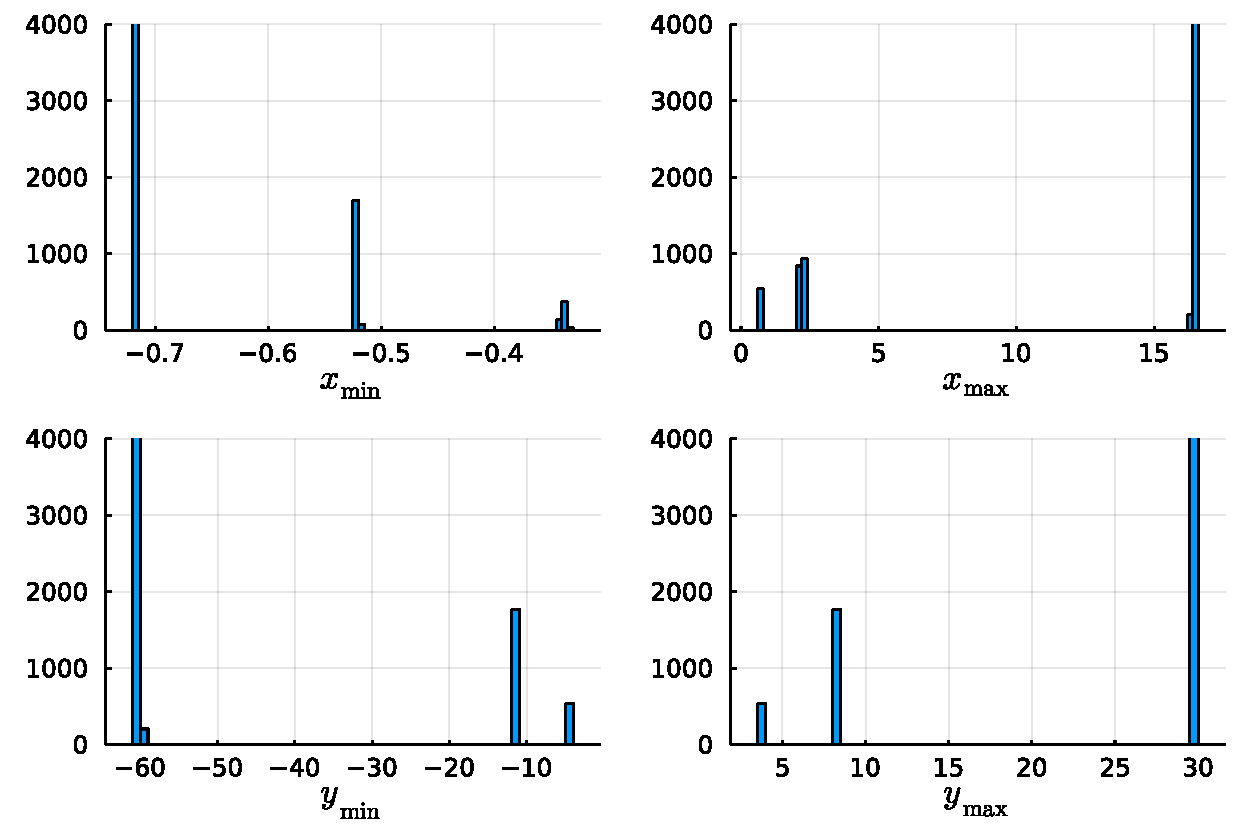
\includegraphics[width=0.8\textwidth]{histograms}
    \caption[Distribution values for local extrema]%
    {Histogram of distribution of values for each local extrema with rate of
        change equal to 1 (tol $1^{-6}$).
    }%
    \label{fig:histograms}
\end{figure}

\begin{table}[H]
    \centering
    \caption{Cluster centers}%
    \label{tab:clusters}
    \begin{tabular}{crrrr}
        \toprule
        Cluster & $x_{\min}$ & $x_{\max}$ & $y_{\min}$ & $y_{\max}$ \\ \midrule
        A & -0.716937 & 16.4835  & -60.2806  & 29.7273 \\
        B & -0.521985 &  2.20031 & -11.3237  &  8.17958 \\
        C & -0.338311 &  0.68522 &  -4.48625 &  3.84119 \\
        \bottomrule
    \end{tabular}
\end{table}

\begin{figure}[H]
    \centering
    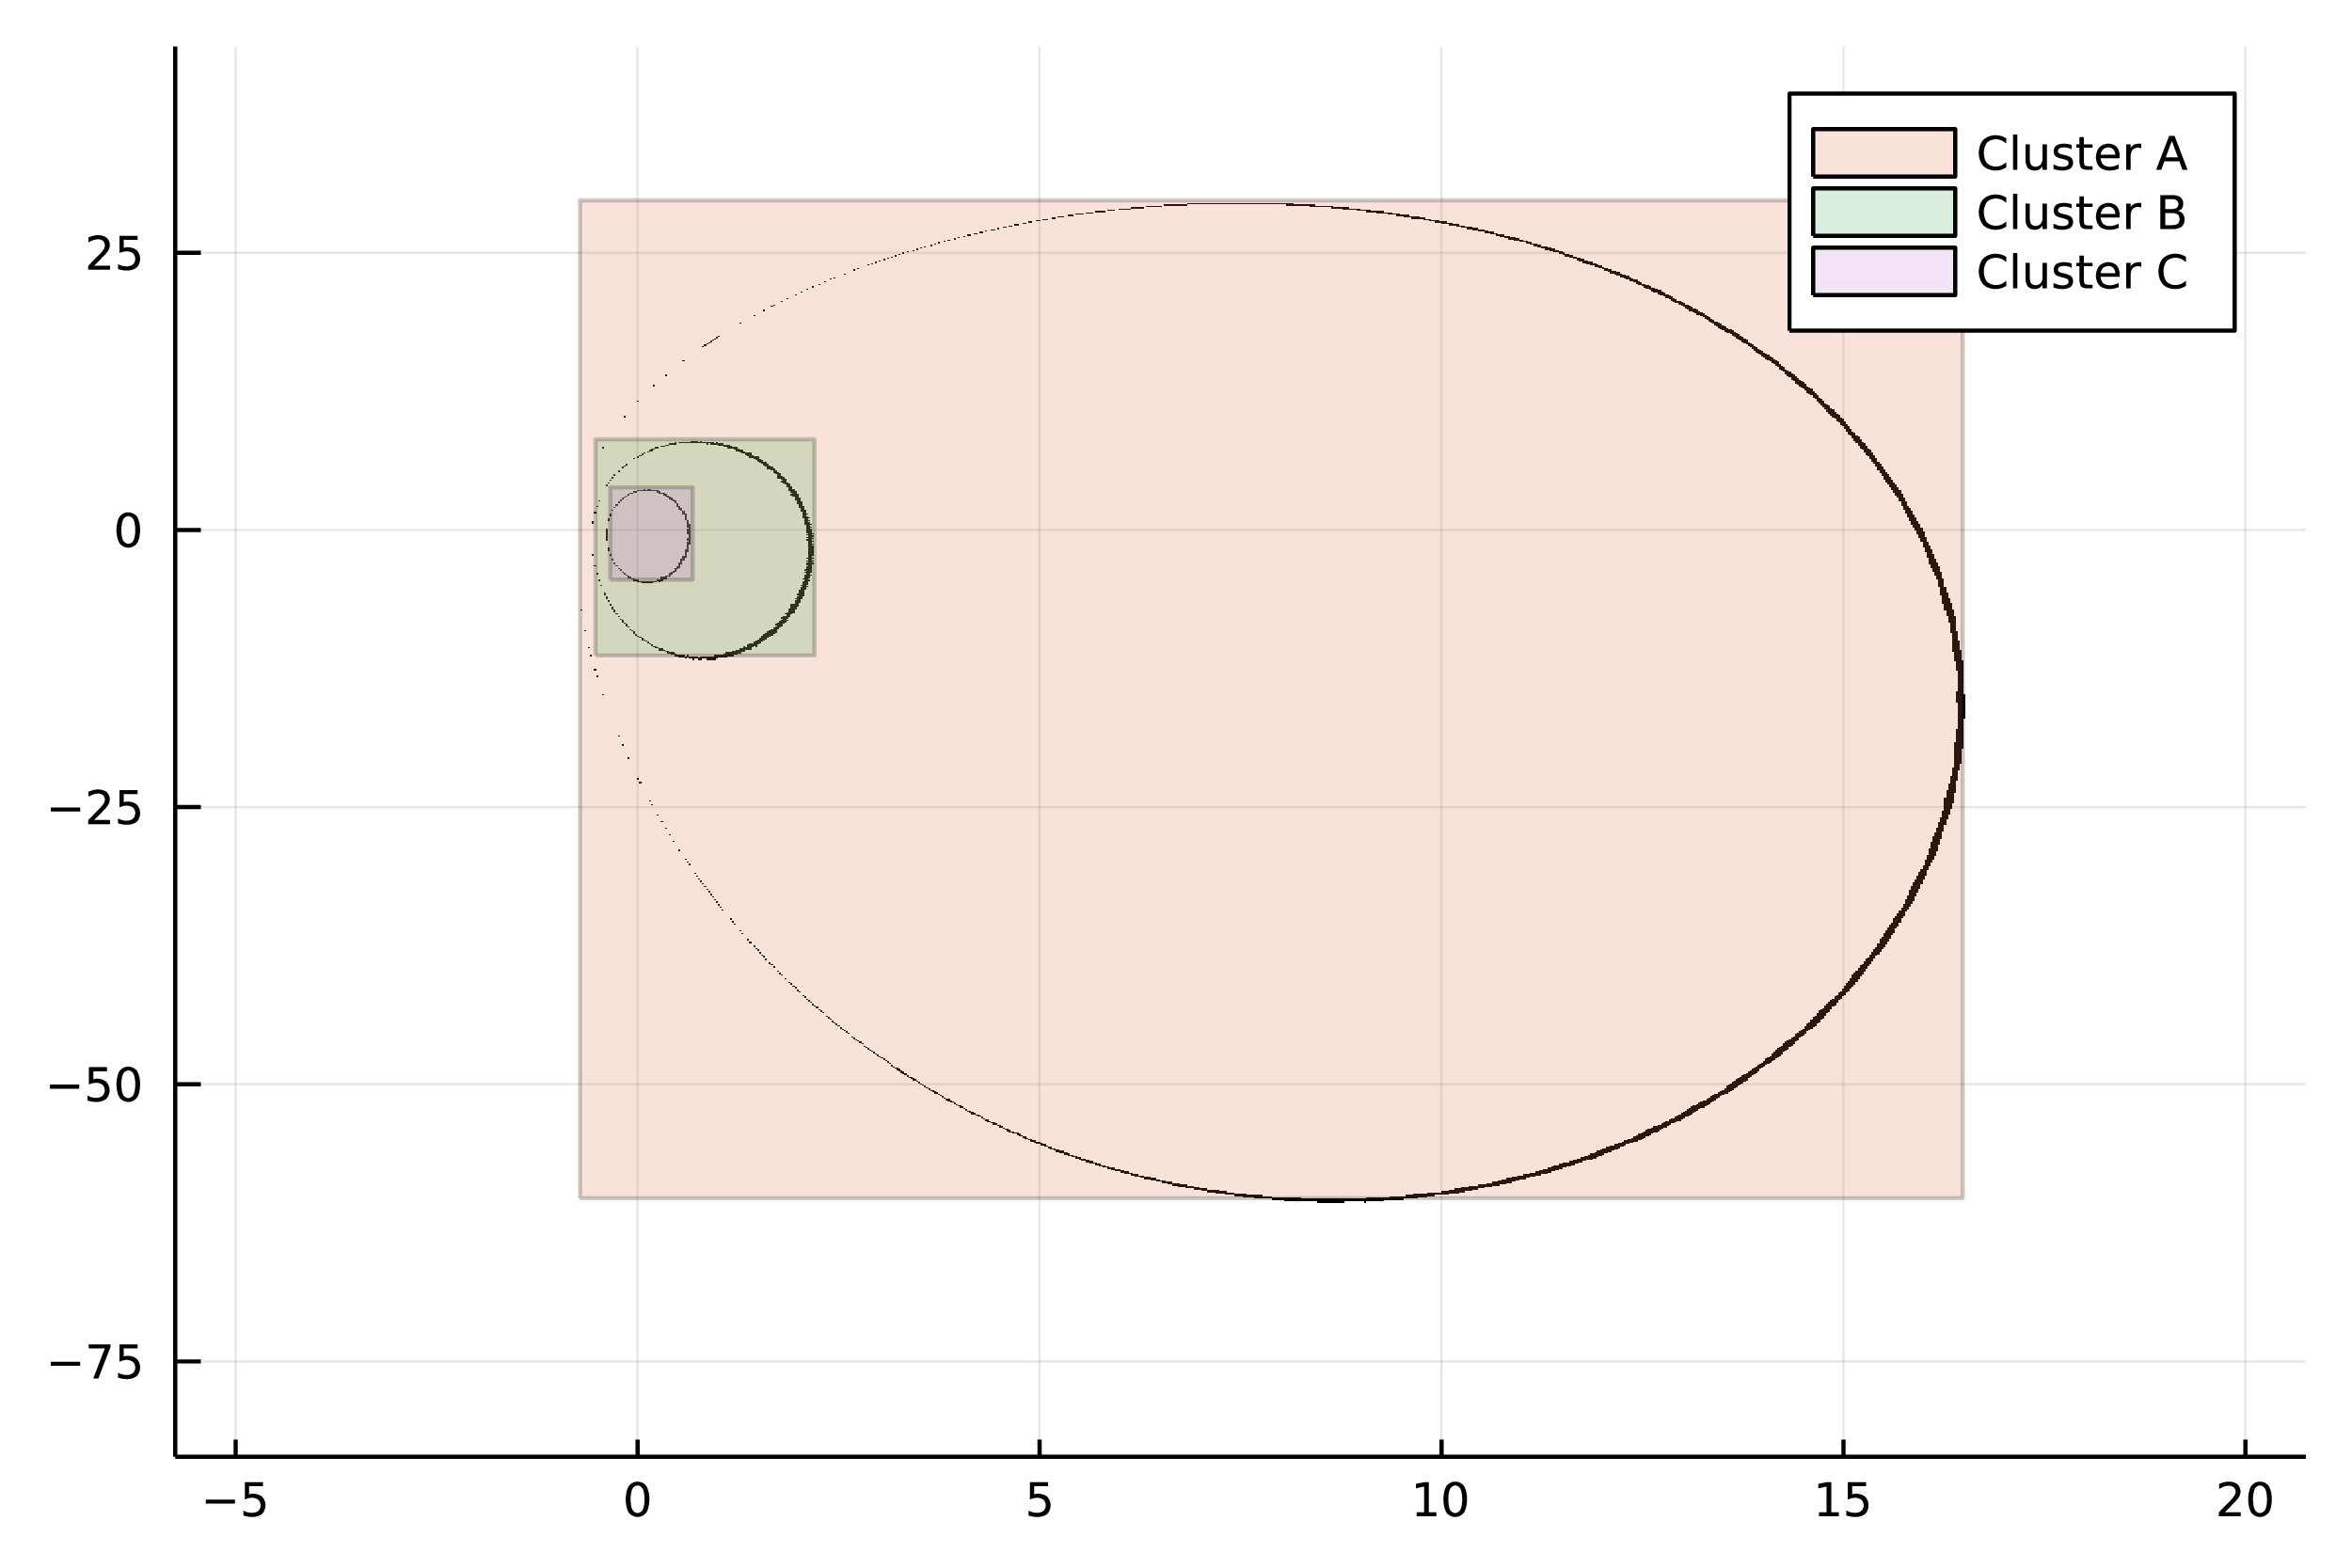
\includegraphics[width=0.8\textwidth]{bounding}
    \caption{Phase portrait. Bounding boxes defined by the clusters in \cref{tab:clusters} overlaid on top of \cref{fig:kuznetsov_cuda}
    }%
    \label{fig:bounding}
\end{figure}

\pagebreak
\subsection{Scanning the values of the coefficients}
% {\bf Improved method???}
% {\bf Scanning the values of the coefficients???}

\Cref{fig:bounding_a10_1} shows the phase portrait used for finding limit cycles in the same system used in the previous examples (\cref{eq:kuznetsov}) but with a slight modification of parameter $a$ from 10 to 10.1. We can see that the cycles are slightly more similar in size. Changing to 10.2 only one cycle remains. With $a = 9.9$ there are only two cycles. Other slight modifications of the other parameters also reduce the number of cycles.

\begin{figure}[H]
    \centering
    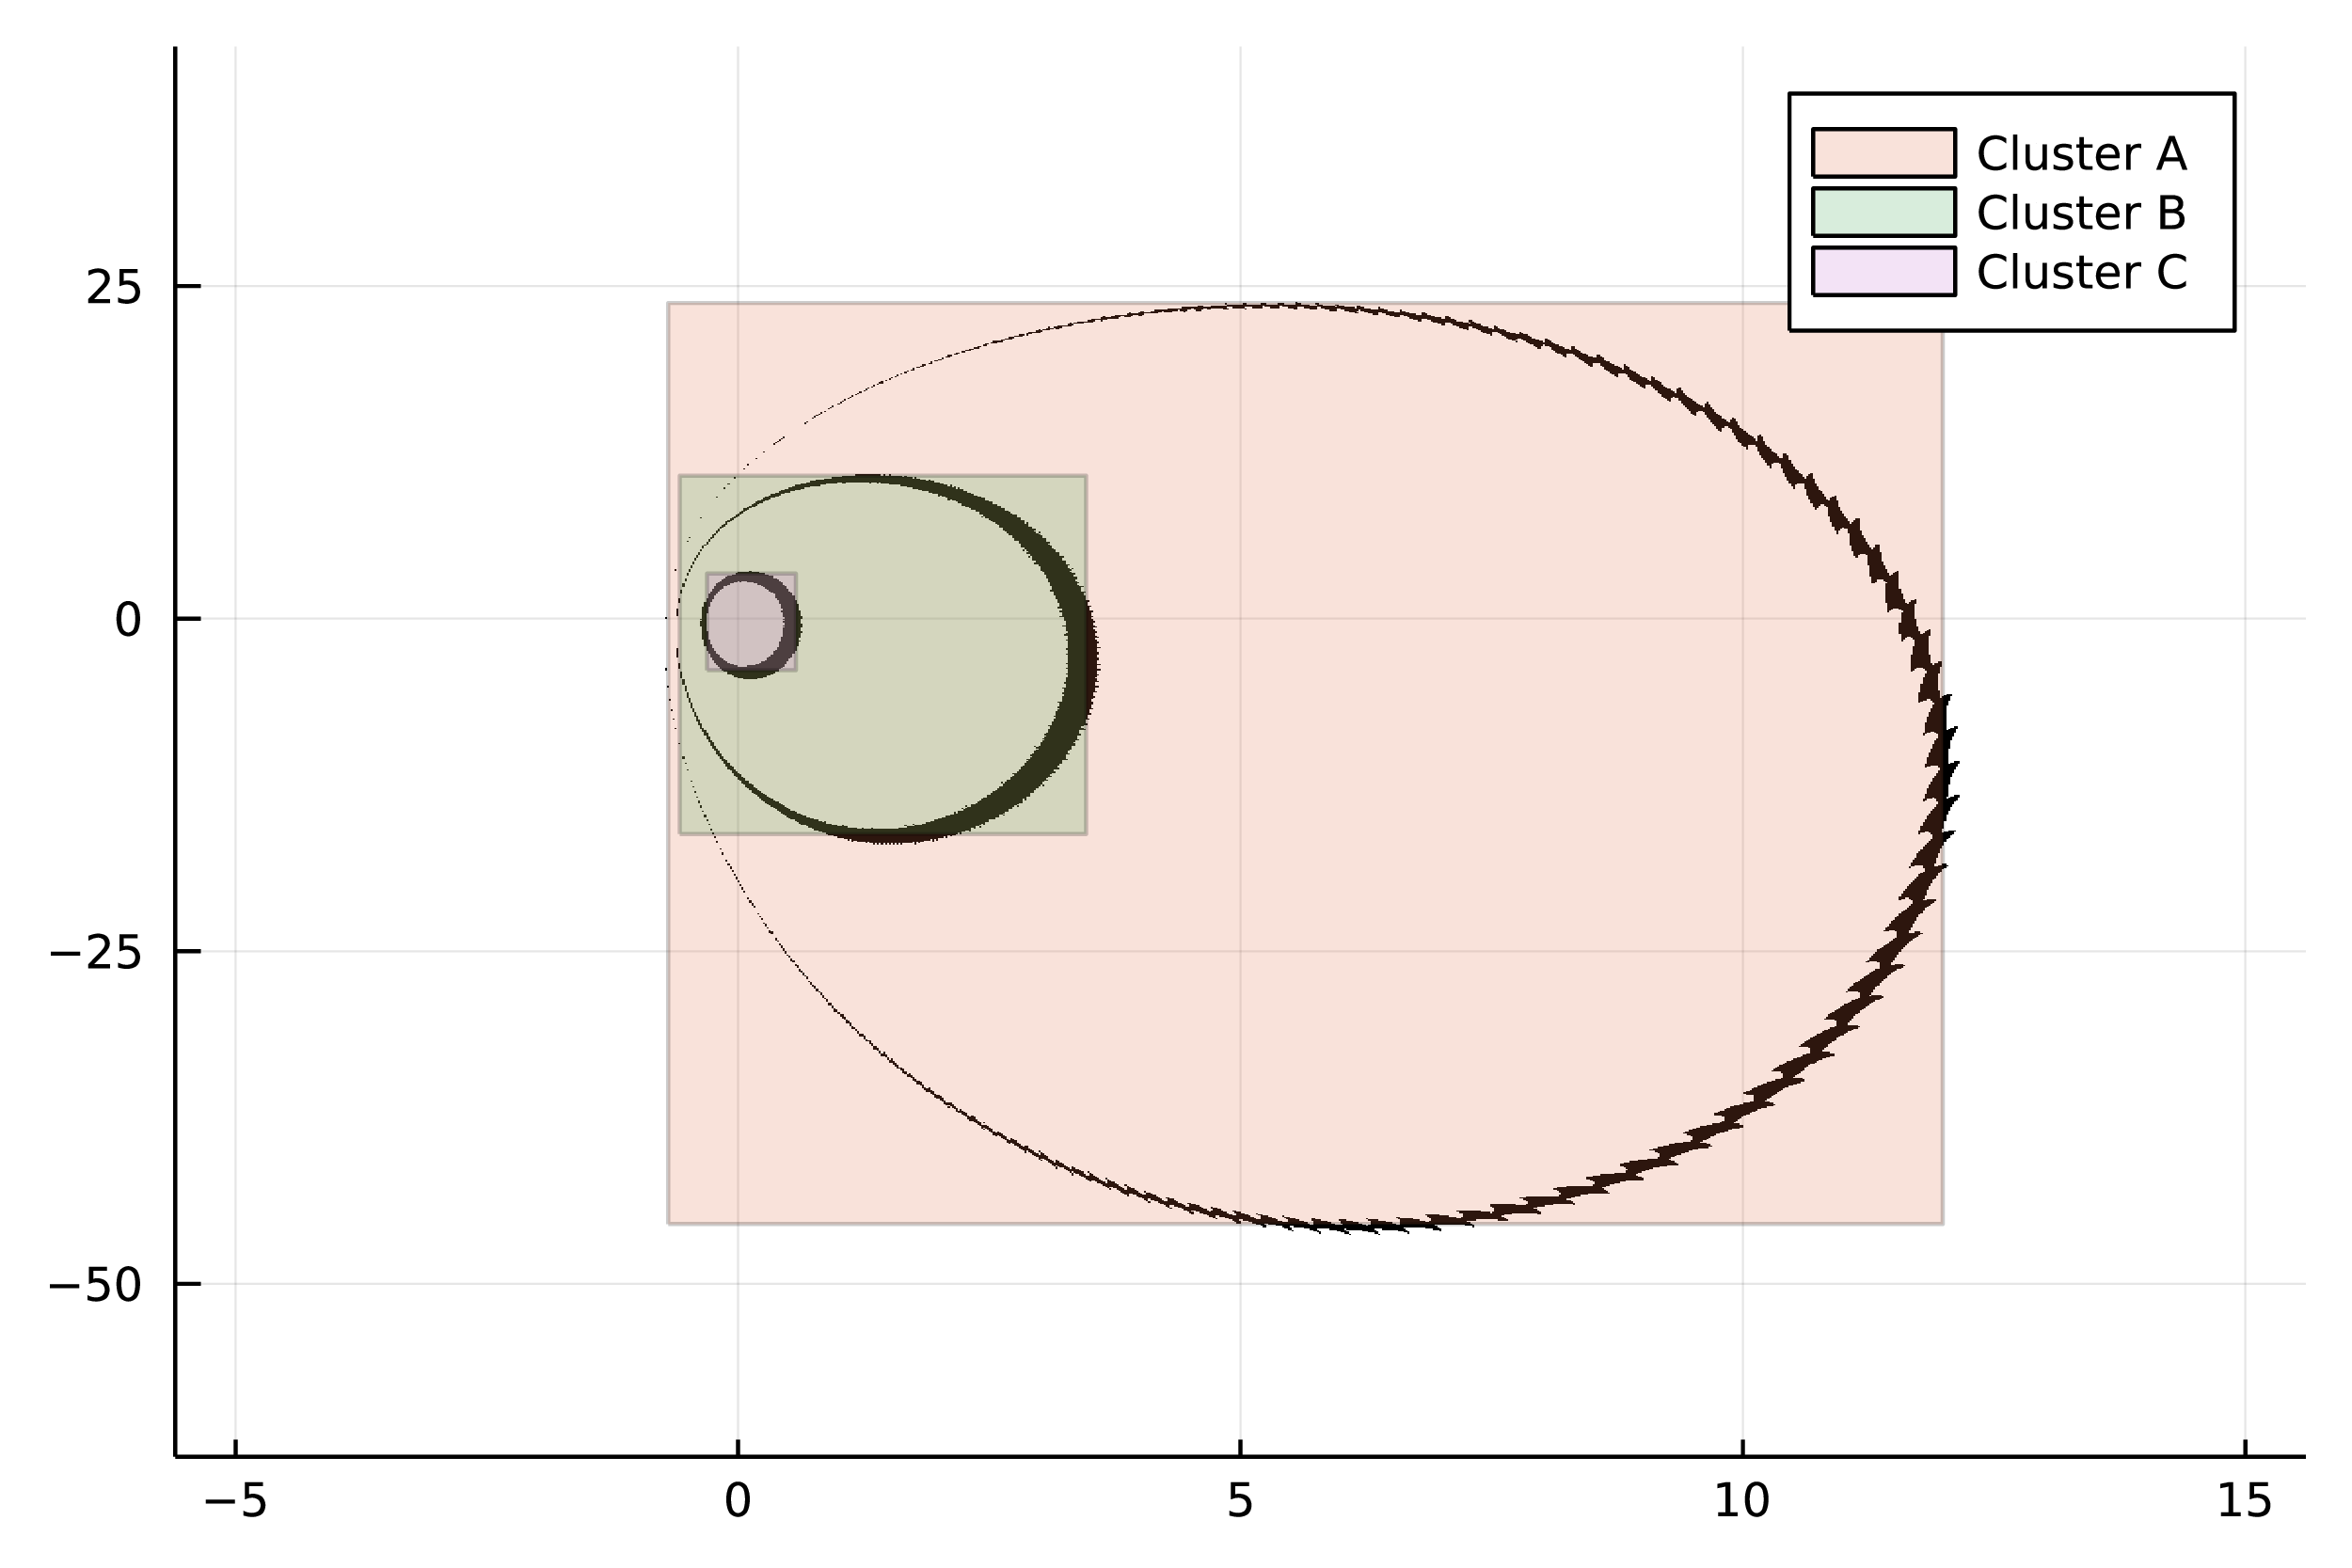
\includegraphics[width=0.8\textwidth]{bounding_a10_1}
    \caption{Phase portrait of the system for parameters as in \cref{eq:kuznetsov} but with parameter $a$ modified from $10.0 \to 10.1$. Three limit cycles are visible.
    }
    \label{fig:bounding_a10_1}
\end{figure}

\pagebreak
\subsection{Changing window range}%
\label{sub:window_range}

One of the important issue is a possible dependence of the number of the limit cycles on the size of the area which is used for searching them. The previous figures were obtained by searching for limit cycles inside a rectangle bound by $x \in (-5, 20), y \in (-60, 40)$. In the following section an analysis on the capacity of the program to find the cycles with different windows will be performed.

\paragraph{Bigger area}

\begin{figure}[H]
    \centering
    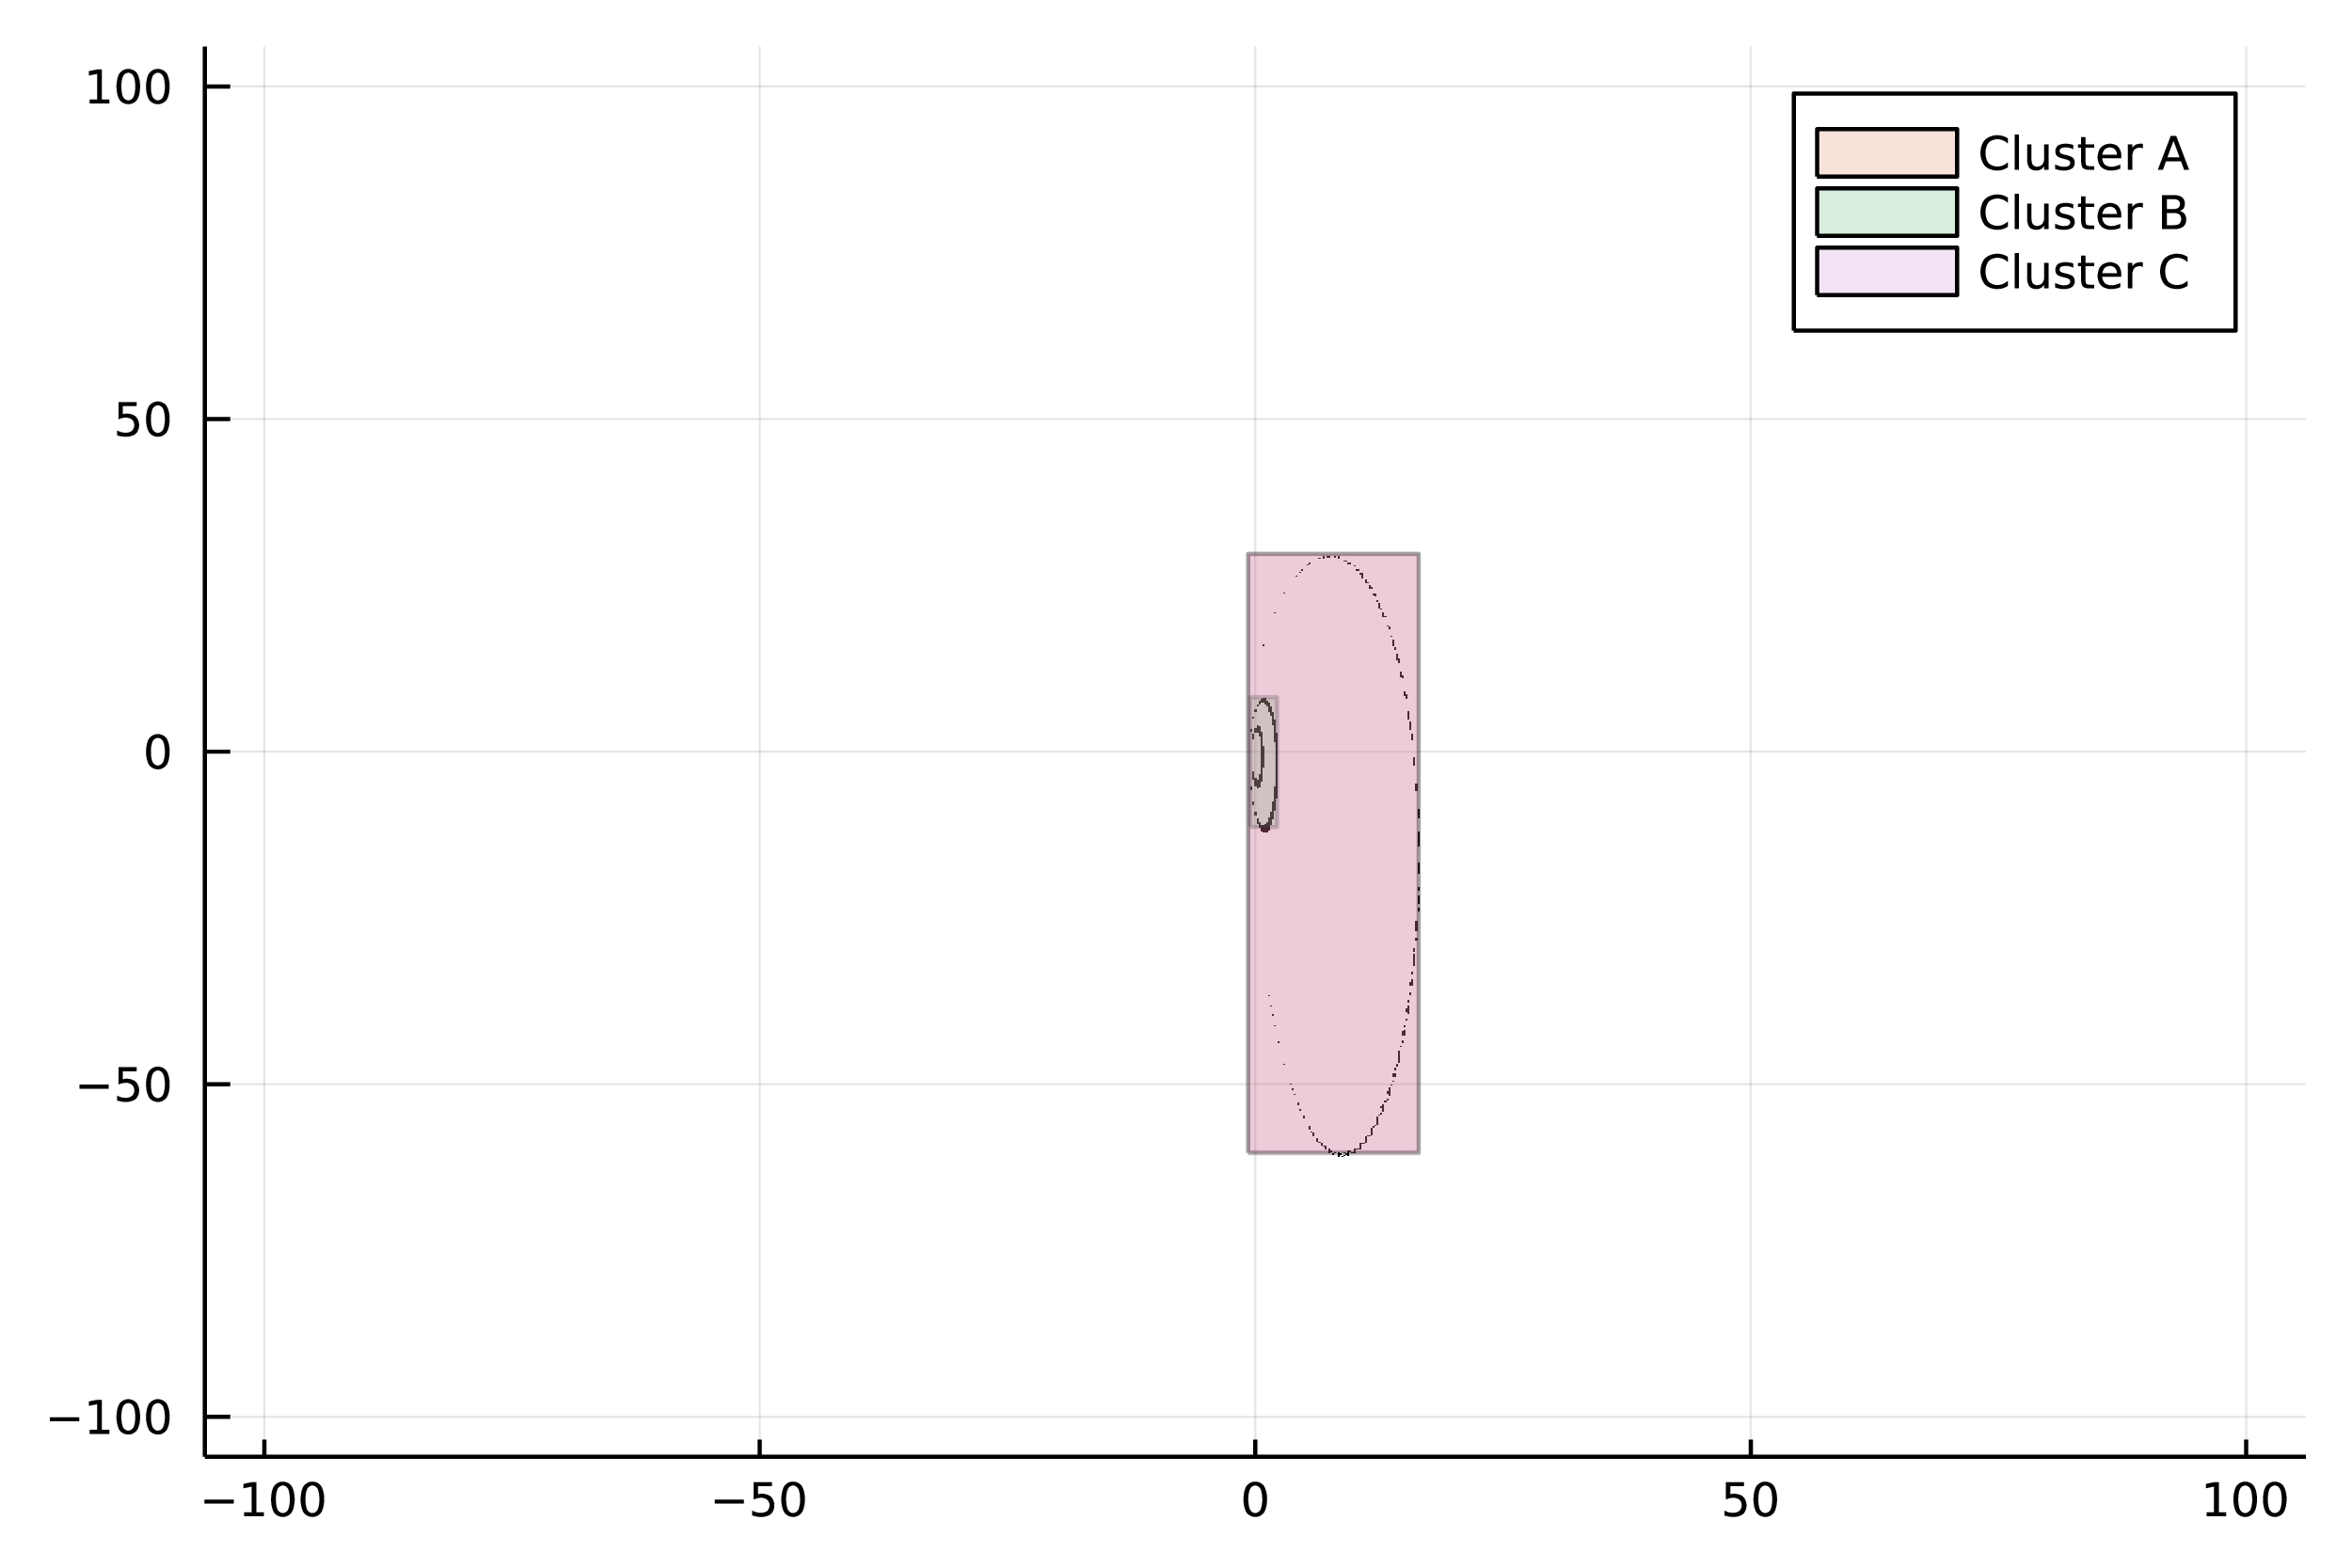
\includegraphics[width=0.8\textwidth]{bounding_100x100}
    \caption{Limit cycles found on system from \cref{eq:kuznetsov} \\
        ($1024 \times 1024$ grid over $x, y \in (-100, 100)$)
    }%
    \label{fig:bounding_100x100}
\end{figure}

As shown in~\cref{fig:bounding_100x100}, with a window of $x,y \in (-100,100)$ we obtain the clusters without problem. Increasing the window further to $(-1000, 1000)$ while maintaining the same
grid size does only find the two bigger limit cycles.
% {\bf report also the grid size}
A possible optimization could be to make two steps: one to find the biggest limit cycles and a second one using as a window the bounding box of the limit found.

\pagebreak
\paragraph{Partial occlusion}

A good algorithm should be robust to partial occlusion of the cycle, meaning that even if part of the cycle is outside the window it should still be detected. In~\cref{fig:bounding_occ} we show an image of the results applied with a window of $x \in (0, 5), y \in (0, 20)$ (Shown in gray). Indeed, the clusters are equivalent to the ones in the previous examples. Note that the line of the biggest cluster is very thin
since there are not many points. As long as the window contains enough part of the trajectory of a limit cycle\footnote{And the trajectory is not stiff (see \cref{sub:stiffness})} with enough resolution, the cycles can be identified.

\begin{figure}[H]
    \centering
    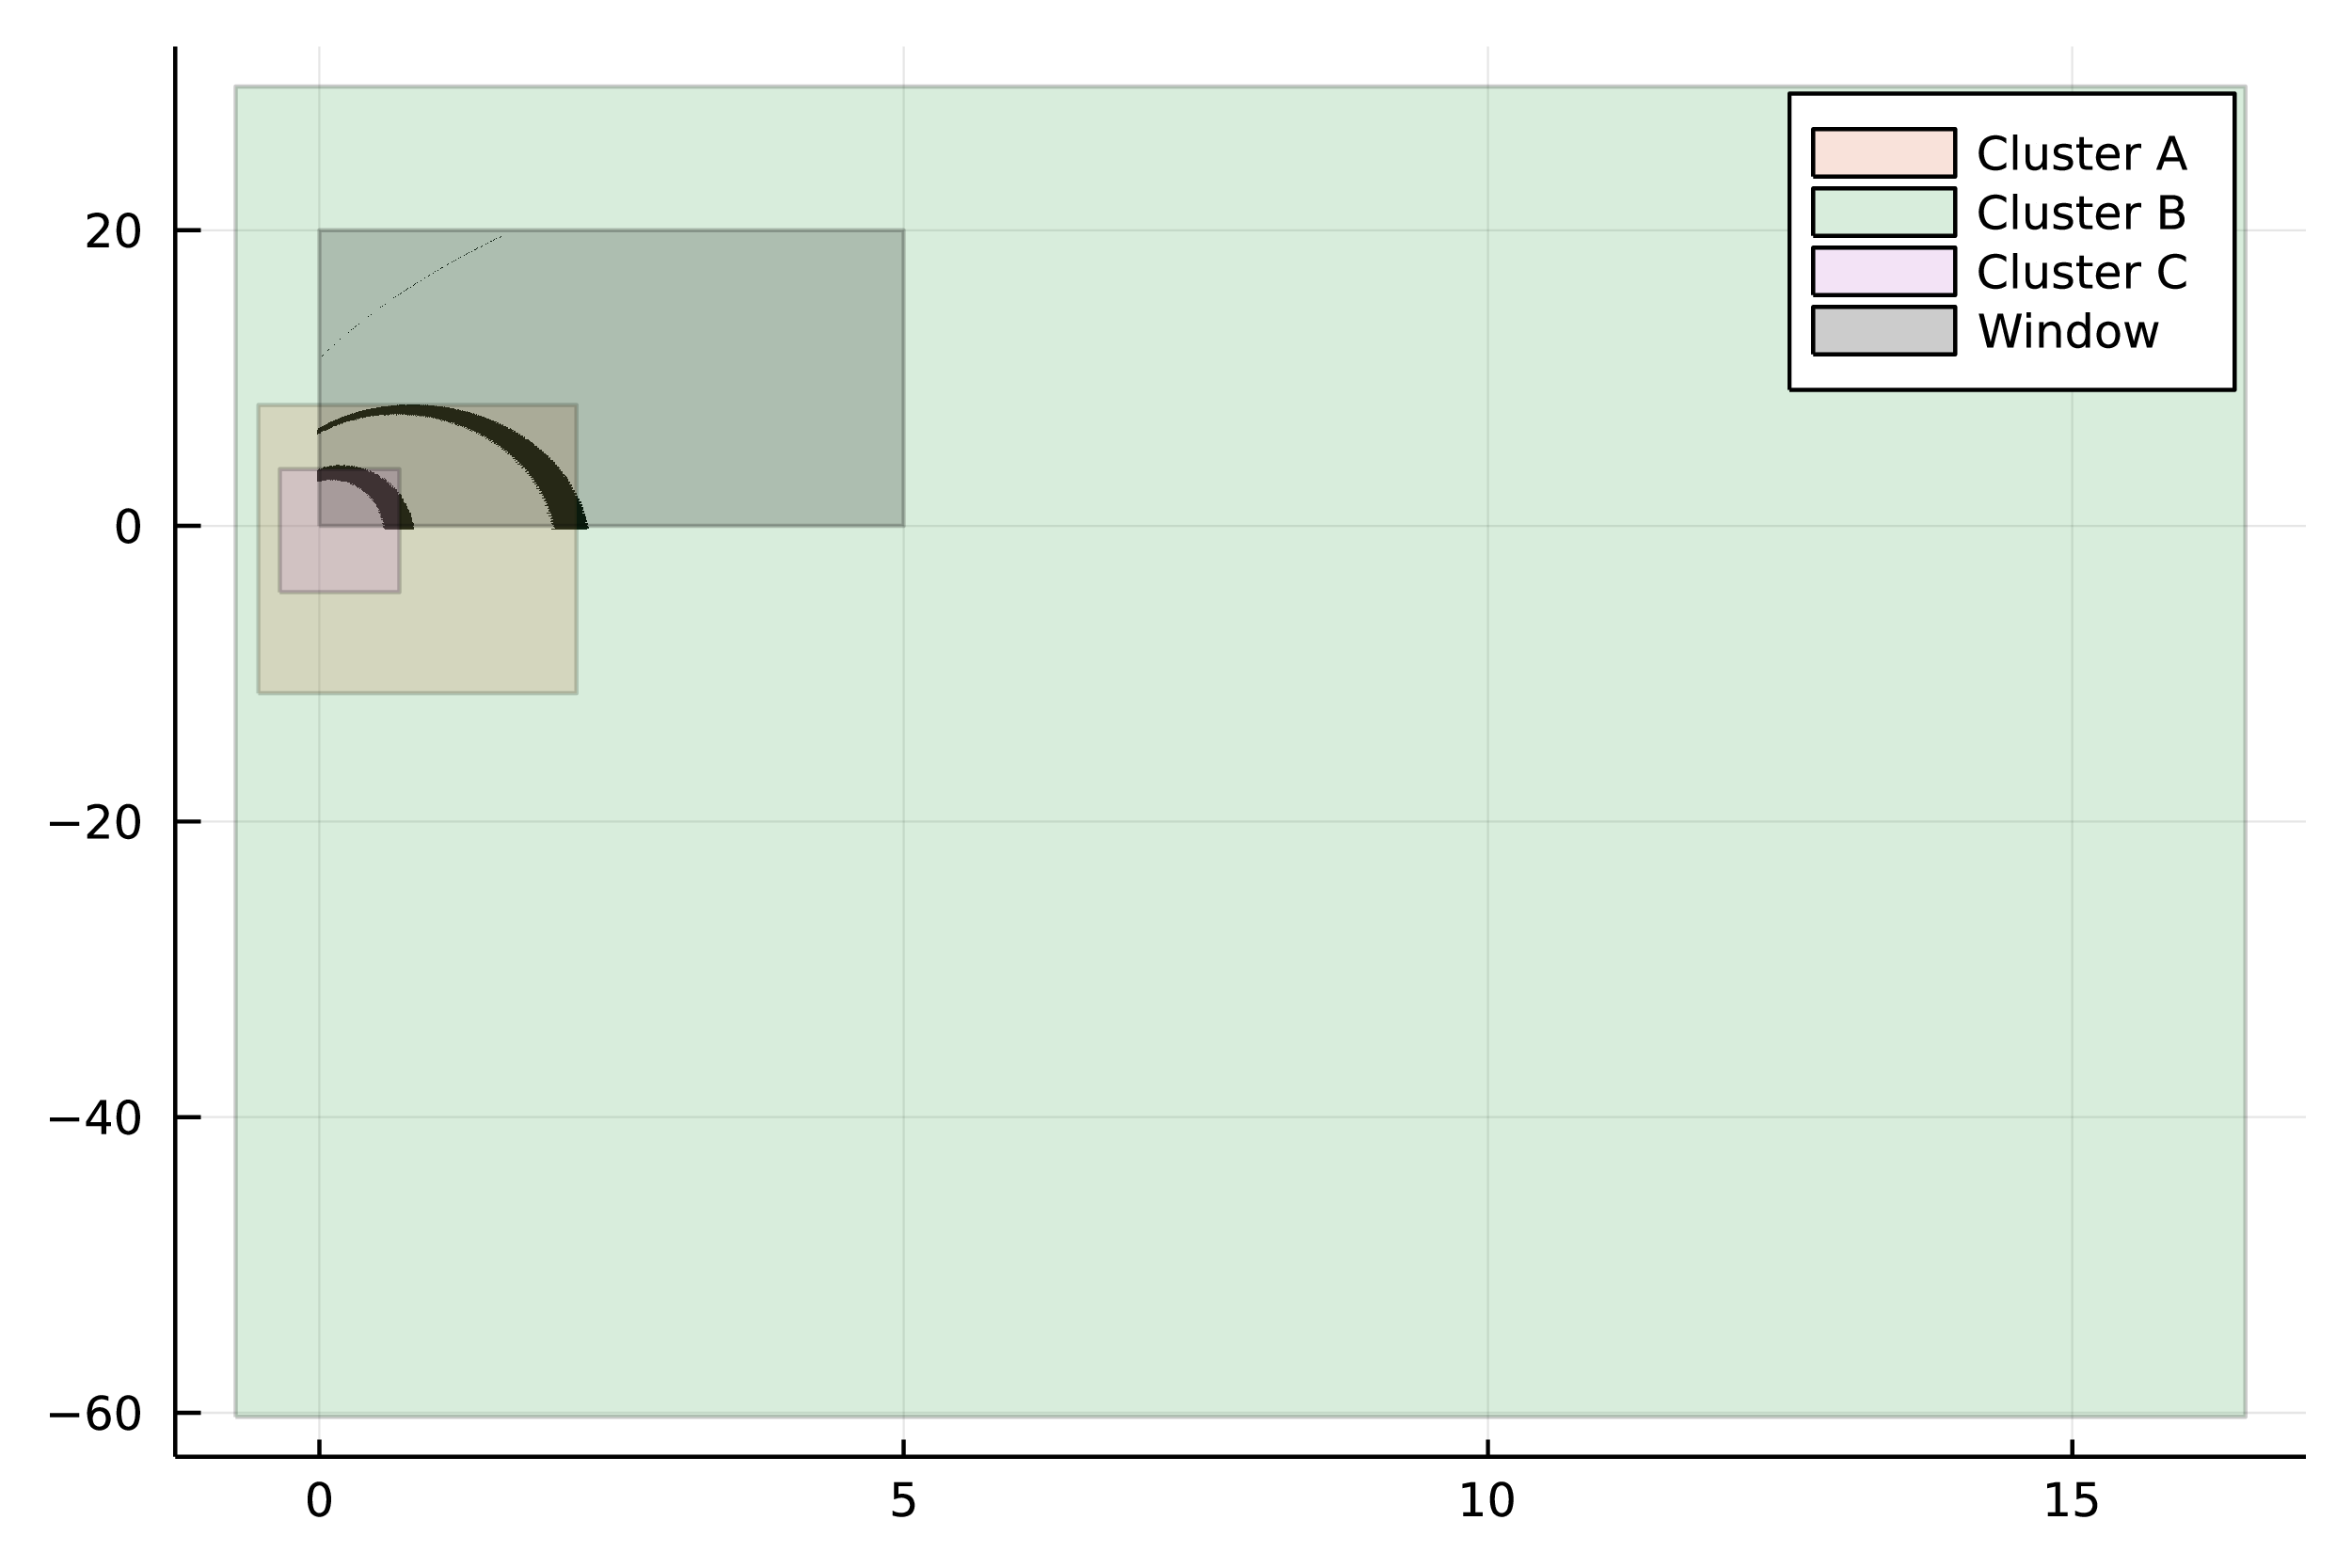
\includegraphics[width=0.8\textwidth]{bounding_occlusion}
    \caption{Limit cycles found on system from \cref{eq:kuznetsov} \\
        ($1024 \times 1024$ grid over $x \in (0, 5), y \in (0, 20)$)
    }%
    \label{fig:bounding_occ}
\end{figure}

\pagebreak
\paragraph{Compactified plane}

Since the $(x,y)$ plane in $\mathcal{R}^2$ is infinite it is not possible to cover it with a finite regular grid. A possible way out is
%in order to visualize limit cycles without restricting portions of the plan a compactification should be performed.
to do a compactification so that the infinitely large plane is mapped to a finite-size box. In \cref{sec:compact-stiff} there is a more in depth explanation of how this can be done. A simple way to perform the compactificaction $(x,y)\to(x',y')$ is to use mapping $x' = \arctan x$, $y' = \arctan y$ where $x\in(-\infty, \infty)$ to $x'\in(-\pi/2, \pi/2)$. This compactification is not ideal as it significantly deforms the plane and does not preserve the angles, but still it allows to perform the search of cycles in essentially infinite phase space.

However, this compactification does not help if they are big since they get
\emph{squished} on the borders meaning that without a very high resolution it is
not possible to find them. For instance, if we divide the range $(-\pi/2,
\pi/2)$ in 4096 parts, in the outermost point before $+\infty$: correspond to
$\tan\left(\pi/2 - \pi/4096\right) \approx 1304$ which is approximately 1304, the
immediately previous value is $\tan\left(\pi/2 - 2\pi/4096\right) \approx 652$. If
our limit cycle does pass between these values it will not be found.

% I'm not sure if it is clear now.
% {\bf ??? and what, why it is a problem, rephrase}.

The result of applying the tangent compactification and running the program is shown
in~\cref{fig:bounding_compact}. The biggest cycle is almost non visible despite the fact that it is not particularly big ($y_{\min} \approx -60, y_{\max} \approx 30$).

\begin{figure}[H]
    \centering
    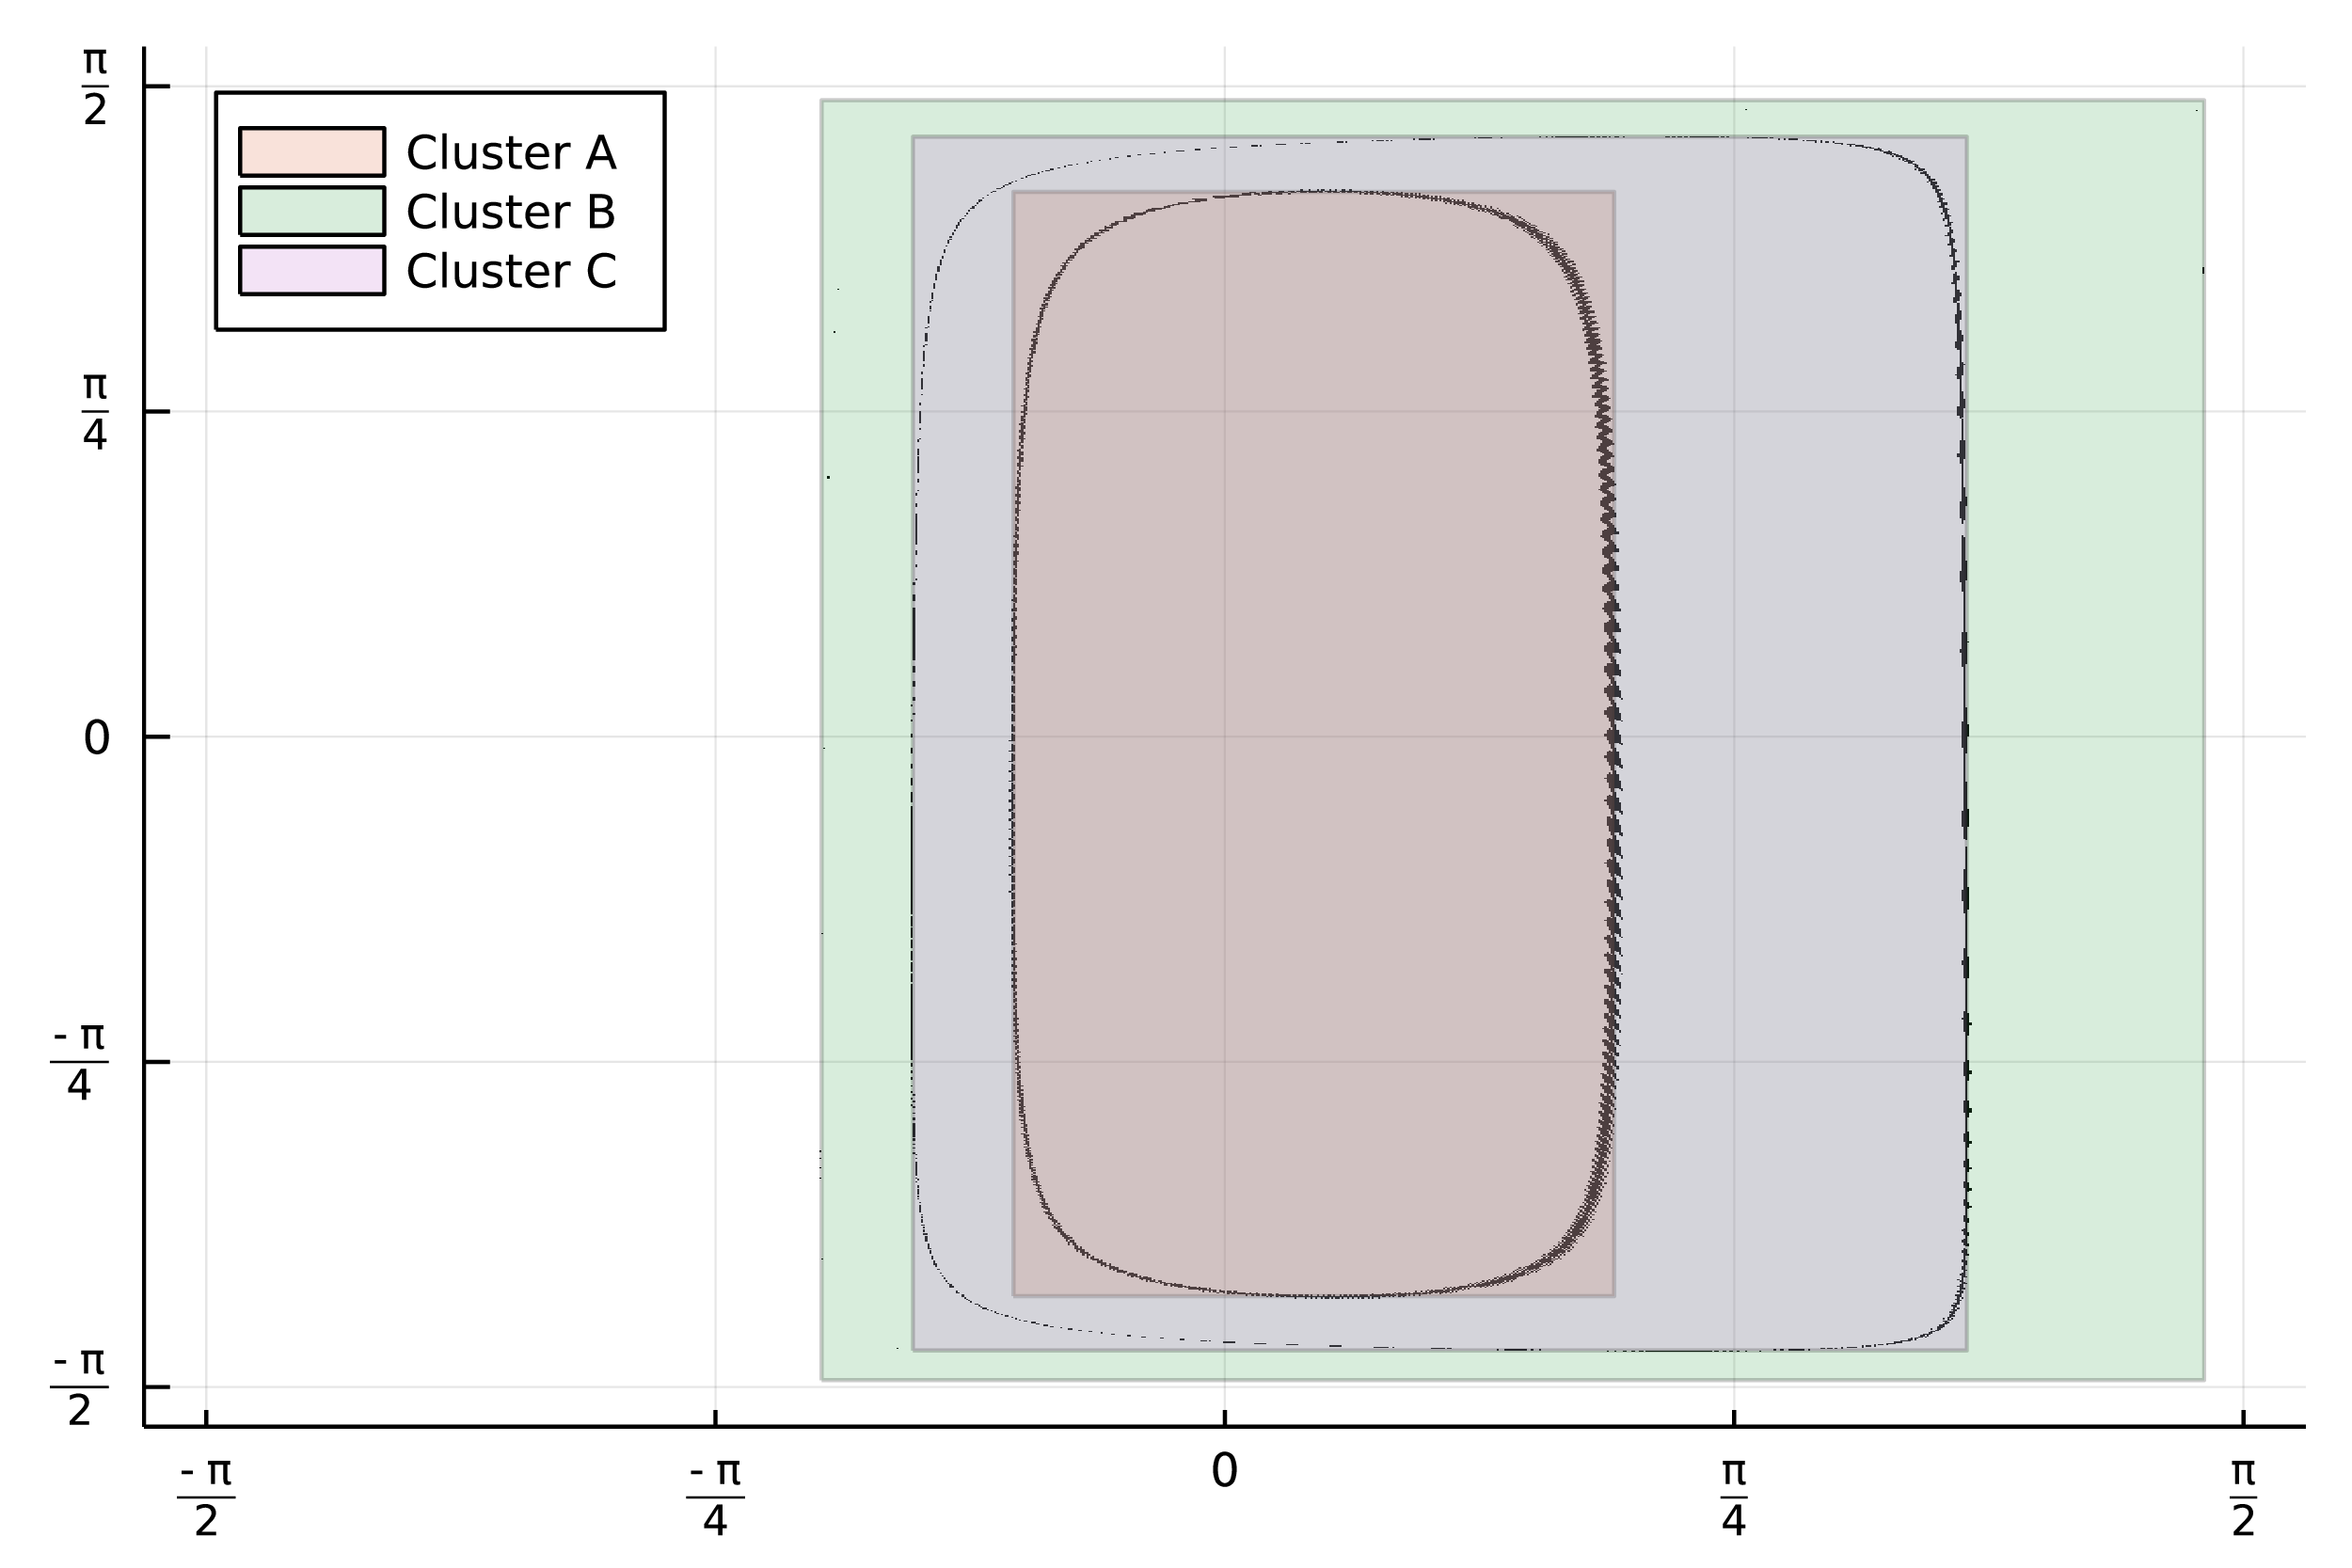
\includegraphics[width=0.8\textwidth]{bounding_compact}
    \caption{Limit cycles found on system from \cref{eq:kuznetsov} \\
        ($1024 \times 1024$ grid over compactified plane)
    }%
    \label{fig:bounding_compact}
\end{figure}
